\documentclass{article}
\usepackage[utf8]{inputenc}
\usepackage{amsmath}
\usepackage{natbib}
\usepackage{parskip}
\usepackage{tikz}
\bibliographystyle{jasa}
\usetikzlibrary{positioning,calc,backgrounds}
\usepackage{thmtools}
\usepackage{lipsum}
%\usepackage{blindtext}
\usepackage{xcolor}
\usepackage{comment}



\title{Notater til masteren}
\author{johaskog }
\date{January 2021}

\parskip 0.2in %making spacing between paragraphs
\newcommand{\dd}{\mathrm{d}}
%\newtheorem{theorem}{Theorem}
\colorlet{myblue}{blue!5!white}
%\definecolor{myblue}{rgb}{188,217,255}
%\definecolor{myblue}{rgb}{1,1,1}

\declaretheorem[
  shaded={rulecolor=black, rulewidth=1pt, bgcolor=myblue},
  name=Theorem,
]{theorem}





\begin{document}

\maketitle
%need this to plot the tikz trees. 
\input{tikz-trees/basics_tikz}


\newpage
%\section{Introduction}
\chapter{Introduction}
Schizophrenia is a psychotic disorder where at least two of the symptoms delusions, hallucinations, disorganized speech, grossly disorganized or catatonic behaviour or negative symptoms such as reduced emotional expressions and lowered motivation, have to be present. 
Delusions are beliefs that will not change if contradicting evidence is presented. The most common type of delusions are persecutory delusions. People that have those kinds of delusions might think that they will be hurt, injured, tormented or so on by others. Referential delusions are also common. Then one are putting meaning into comments, gestures and actions, thinking that they are about oneself, when they not necessarily are. Completely improbable beliefs are called bizarre delusions. These are delusions others find far-fetched, and they are things that cannot happen in real life. A bizarre delusion could for example be that a person believes that their organs have been removed replaced by someone else's organs without there being any scars or other evidence of that happening. A delusion that is not bizarre could be that you think you are under police surveillance without there being any evidence of that. It might be hard to distinguish between delusions and strongly held ideas. The main distinction is about the degree of conviction, and how much or little the beliefs can be amended when contradicting facts are presented \citep{dsm-5}. 
%Hallucinations are sensory impressions that happen without any external stimulus. Hence, others usually does not experience the same impressions. The hallucinations are perceived as normal experiences to the person having them. For schizophrenic people, they often occur as voices which can be distinguished from the persons own thoughts. 
%Disorganized speech means that one are switching between topics rapidly and giving unrelated answers to questions. 
%Grossly disorganized behavior is also referred to as abnormal behavior, and catatonic behavior means that one has a dampened reaction to things happening around oneself. (All of the above is from DSM-5).


Delusions are one of the main characteristics of schizophrenia as it appears in about three out of four of those diagnosed \citep{garety2011}. Researchers have been trying to understand how the delusions are formed and maintained in order to improve treatment \citep{dudley_meta_2016}. One important finding is that deluded individuals seem to make decisions based on less evidence than both healthy and psychiatric controls. This is often referred to as a "jumping to conclusions" (JTC) bias \citep{dudley_meta_2016}. A person with this bias might reach decisions or form beliefs before reaching realistic conclusions, and thus accept unrealistic ideas. They are therefore more prone to delusions \citep{dudley_meta_2016}. The hope is that if we can detect the JTC bias, we can reduce the delusional thinking, and thus prevent delusions \citep{dudley_meta_2016}.

The JTC bias is traditionally tested with a probabilistic reasoning task called the beads task. The participants are presented with two jars containing beads of two colours, for example red and blue. The two jars have opposite ratios of each colour, meaning that if the first have 85\% red beads and 15\% blue, the second has 15\% red and 85\% blue beads. The participants are told that beads are drawn from one of the jars, and their task is to find out which one that is. They are told to choose only when they are completely sure, and they draw as many beads as they want. The beads are drawn sequentially, and after each draw the participants are asked if they want to choose which jar beads are drawn from or if they want to draw more beads. One are usually said to have a JTC bias if one decides after one or two beads \citep{moritz2017}. However, the beads task has shown to pose some problems.

Some of the first to use the beads task were \citet{huq1988}. Already in that article they presented some of the problems with the beads task. They used an 85-15 ratio of the beads. When the two first beads that are drawn are of the same colour, it is a 97\% probability that the beads are from the jar with 85\% of the beads in that colour. One might therefore argue that choosing jar at that point is reasonable, and that it does not show a JTC bias. Deluded individuals make decisions earlier that the control groups, but \citeauthor{huq1988} argue that non-deluded individuals are more conservative, and that people with delusions simply cancel out that bias when gathering less information. In an article by \citet{moritz2017}, other problems with the beads task are discussed. For example that many participants seem not to understand that all the beads are drawn form the same jar. This makes them think that after each bead is drawn, they have to guess which jar that bead is drawn from. These participants are then classified to have a JTC bias. We can also see that it is common to make logical errors due to miscomprehension. In an article by \citet{moritz2005}, they found that 52\% of the schizophrenic participants and 23\% of the healthy controls had at least one response that was not logical. The participants that misunderstand are more likely to choose early. \citet{moritz2017} further states that the beads task is correlated with intelligence. Lack of intelligence might be a reason for or a confound for misunderstanding the task. It is also stated that confidence influences decision-making. The participants are asked to choose when they are completely sure which jar the beads are drawn from, which could make more confident participants decide earlier. We might also conclude that hasty decisions are made because the participants like to take risks or that they are not cautious, or both. However, other tasks that accounts for confidence also display a JTC bias with the delusion-prone participants. Additionally, there is only a one-dimensional sequence of events in the beads task. Thus, it is harder to find different versions to test multiple times. 

The box task has been suggested as an alternative to the beads task. Here, the participants are presented with a grid of a fixed number of boxes. When a box is opened, one out of two colours is displayed, for example blue and red. The participants are told that one of the colours are always in majority, and their task is to find out which one \citep{moritz2017}. They can open as many boxes as they want before they make a decisions. Both the number of boxes and the ratio of the two colours can be changed for each new trial. 

In this report we model how the participants make decisions in the box task. In the version of the box task used here, there are twelve boxes. We use two different versions of the box task. The first one is an unlimited one, where the participants can open as many boxes as they want, even until all twelve boxes are opened, before reaching a decision. In the second version, the participants are told that the test will terminate at a random point. If the test terminates before the participant has decided what the majority colour is, this counts as a failed trial. We call this the limited version. In Figure \ref{picture_of_box_task}, we see a limited trial of the box task with red and blue boxes. The participant have opened two boxes, and has to choose whether to open another box or to choose that either blue is the dominant colour, or that red is. 

\begin{figure}
    \centering
    \includegraphics[scale=0.486]{Sections/Box task 2.png}
    \caption[A Limited Trial of the Box Task Visualised]{Describe the figure}
    \label{picture_of_box_task}
\end{figure}

We have data from 76 participants that have done 10 trials each of the box task. The first trial was a practice trial of the limited version followed by three unlimited and six limited trials. We can model the decisions the participants make using a Softmax model, and fit this model to each participant with maximum likelihood estimation. Thus, we find the maximum likelihood estimates in the Softmax mode. Then, we find confidence intervals for each of these estimates using parametric bootstrapping and percentile intervals. 

As an input in the Softmax model we have an Ideal observer solution of the box task. An Ideal observer is a participant that always makes optimal, or ideal, choices, and thus finds the best solution \citep{idealObs}. Each time a box is opened, the participant have three options. The first is to choose that blue is the majority colour, the second that red is, and the third option is to open another box. For each of these alternatives we have defined loss functions, which represent the cost of choosing the different options. An Ideal Observer would always choose the alternative with the least loss, and would end up with the overall optimal or ideal solution. In this report we are assuming that the total number of red boxes is binomially distributed with parameters 12 and some probability $\theta$. Each time a box is opened, the probability that the box is red is $\theta$ and $1-\theta$ that the box is blue. We also assume a beta prior for $\theta$ with parameters $\gamma$ and $\kappa$. If we have any prior beliefs about the probability of the different colours, this knowledge can be incorporated here. If both $\gamma$ and $\kappa$ is one, this is a uniform prior, meaning that $\theta$ has the same probability of being each possible value between zero and one. 



%(something about: here they are not said to answer when they are completely sure? compared to the beads task, where they are said to answer when comp sure. Jeg klarer ikke å finne ut hvor det står??)


In this report we will firstly go through some of the background theory used later on. Then, we will formulate the model for the decisions the participants make. That includes finding an Ideal Observer solution of the box task, and describing how to find parameter estimates and confidence intervals. Further on we will present some results, both the Ideal Observer solution and the parameter estimated with their respective confidence intervals. Lastly, we have some closing remarks. 
\newpage
\chapter{Background Theory}
%\section{Theory}
In this section we will go through some of the statistical theory used in this thesis. That includes the theorem of total probability, Bayes' theorem, the beta and gamma functions, Bayesian modelling, loss functions, the Softmax function, maximum likelihood estimation and bootstrapping.  

\section{The Theorem of Total Probability}
The theorem of total probability can be used when we have dependent variables and we wish to find the probability of one variable alone(?).
\begin{theorem}[Theorem of Total Probability, Continuous Variables]
If we have a continuous variable, $\Theta$, and a discrete variable, $U$, and both $P(U=u|\Theta=\theta)$ and  $f_\Theta(\theta)$ exist for all $\theta$, then we can find $P(U=u)$ using these \citep{schay2016introduction}. 
\begin{equation}
    \label{lawoftotprob}
    P(U=u) = \int_{-\infty}^{\infty} P(U=u|\Theta=\theta)f_{\Theta}(\Theta=\theta) \: \dd \theta.
\end{equation}
\end{theorem}

\begin{comment}
In \citet{schay2016introduction}, the theorem of total probability for continuous variables is stated as 
\begin{theorem}[Theorem of Total Probability, Continuous Versions]
 For a continuous random variable Y and any event A, if $f_{Y|A}$ and $f_Y$ exists for all y, then
\begin{equation}
   % \label{lawoftotprob}
    P(A) = \int_{-\infty}^{\infty}
    P(A|Y=y)f_Y(y) dy.
\end{equation}
\end{theorem}
\end{comment}




Consider, for example, two discrete random variables $U$ and $V$ that are conditionally independent given the continuous stochastic variable $\theta$. To find the probability that $U+V$ is equal to some integer $j$, we can use the theorem of total probability to condition on theta. Thus,
\begin{equation*}
    P(U+V=j) = \int_{-\infty}^\infty P(U+V=j|\Theta=\theta)f_{\Theta}(\Theta=\theta) \: d\theta
\end{equation*}
Later, we can exploit the conditional independence. If $\theta$ is a probability that is defined on the interval (0,1), this will be integrated on that interval, such that 
\begin{equation*}
    P(U+V=j) = \int_{0}^1 P(U+V=j|\Theta=\theta)f_{\Theta}(\Theta=\theta) \: d\theta.
\end{equation*}
Mer utfyllende her?




\section{Bayes' Rule}
Bayes' rule can be used to find conditional probabilities and distributions. 
\begin{theorem}[Bayes' Rule]
Consider two events, $A$ and $B$. We can find the probability of $A$ given event $B$ by the use of the probability of event $B$ given $A$ and the probabilities of the events $A$ and $B$ separately \citep{statinf}. Hence,
\begin{equation}
\label{bayesrule}
    P(A|B)=\frac{P(B|A)P(A)}{P(B)}.
\end{equation}
\end{theorem}




\begin{comment}
From \citet{schay2016introduction}, we have a version of Bayes' theorem for continuous variables which is stated as 
\begin{theorem}[Bayes' Theorem]
\label{bayestheorem}
For a continuous random variable Y and any event A with nonzero probability, if $P(A|Y=y)$ and $f_Y$ exist for all $y$, then
\begin{equation}
    \label{bayestheorem_eq}
    f_{Y|A}(y) = \frac{P(A|Y=y)f_Y(y)}{\int_{-\infty}^{\infty}P(A|Y=y) f_Y(y) dy}.
\end{equation}
Here $f_Y$is called the prior density of $Y$, and $f_{Y|A}$ its posterior density, referring to the fact that these are the densities of $Y$ before and after the observation of $A$. 
\end{theorem}

From \eqref{lawoftotprob} we see that the denominator is the probability of event $A$, \begin{equation*}
    \int_{-\infty}^{\infty}P(A|Y=y) f_Y(y) = P(A),
\end{equation*}
such that Bayes' theorem can be stated as
\begin{equation}
    \label{bayestheorem_eq2}
    f_{Y|A}(y) = \frac{P(A|Y=y)f_Y(y)}{P(A)}.
\end{equation}


Or:
\end{comment}

\begin{comment}
\begin{theorem}[Bayes' Theorem]
\label{bayestheorem}
Consider two continuous random variables, $U$ and $\Theta$, that both have a nonzero probability. If both $P(U=u|\Theta=\theta)$ and $P(\Theta=\theta)$ exist for all $\theta$, then 
\begin{equation}
    \label{bayesrule}
    P(\Theta=\theta|U=u) = \frac{P(U=u|\Theta=\theta)P(\Theta=\theta)}{\int_{-\infty}^{\infty} P(U=u|\Theta=\theta)P(\Theta=\theta) \: \dd \theta}.
\end{equation}
$P(\Theta=\theta)$ is the prior probability/density of $\Theta$, and it represents the prior knowledge we have about that parameter. $P(\Theta=\theta|U=u)$ is called the posterior of $\Theta$, which is the probability density after we have observed that $U=u$ \citep{schay2016introduction}. 
\end{theorem}


From \eqref{lawoftotprob} we see that the denominator is the probability that $U=u$,
\begin{equation*}
    \int_{-\infty}^{\infty} P(U=u|\Theta=\theta)P(\Theta=\theta) \: \dd \theta = P(U=u).
\end{equation*}
Thus, Bayes' theorem can be reformulated as
\begin{equation}
    \label{Bayesrule2}
     P(\Theta=\theta|U=u) = \frac{P(U=u|\Theta=\theta)P(\Theta=\theta)}{P(U=u)}.
\end{equation}


As an example, consider a random variable $U$ that is binomial distributed with parameters $n$ and $\theta$. Thus,
\begin{equation*}
    U|\theta \sim \mathrm{Binomial}(n,\theta).
\end{equation*}
Using Theorem \ref{bayestheorem} and \eqref{Bayesrule2}, we get that the posterior probability of $\Theta|U$ is
\begin{equation*}
    P(\Theta=\theta|U=u) = \frac{P(U=u|\Theta=\theta)P(\Theta=\theta)}{P(U=u)}.
\end{equation*}

\end{comment}

As an example, consider a discrete random variable, $U$. We can find the probability that $U$ is 7 and condition on it being different from 6 by using \eqref{bayesrule}. Thus
\begin{equation}
    P(U\geq 7|U\neq6) = \frac{P(U\neq6|U\geq7)P(U\geq7)}{P(U\neq6)}.
\end{equation}

\section{The Beta and Gamma Functions}
%The beta distribution is continuous on the interval between 0 and 1, and have two parameters \citep{statinf}. Consider a parameter $\theta$ is beta distributed with parameters $\gamma$ and $\kappa$, hence,
%\begin{equation*}
%    \theta \sim beta(\gamma,\kappa).
%\end{equation*}
%The probability density function of $\theta$ is then
% \begin{equation}
    % \label{betadistribution}
    % f(\theta|\gamma,\kappa) = \frac{1}{\mathrm{B}(\gamma,\kappa)} \theta^{\gamma-1}(1-\theta)^{\kappa-1},\:\: 0<\theta<1, \gamma>0, \kappa>0,
% \end{equation}
% where $\mathrm{B}(\gamma,\kappa)$ is the beta function, meaning that


Later, we will use the beta and gamma functions and some properties of these, thus, these are stated here. This theory can for example be found in \citet{statinf}. The gamma function for a parameter $\kappa$ is 
\begin{equation*}
    \label{gamma_func}
    \Gamma(\kappa) = \int_0^\infty t^{\kappa-1}e^{-t} \dd t.
\end{equation*}
A useful property of the gamma function is that it is recursive. Hence,
\begin{equation*}
    \Gamma(\kappa+1) = \kappa \Gamma(\kappa), \quad \kappa>0 .
\end{equation*}

Additionally, the beta function with parameters $\gamma$ and $\kappa$ is defined as
\begin{equation*}
    \mathrm{B}(\gamma,\kappa) = \int_0^1 \theta^{\gamma-1}(1-\theta)^{\kappa-1} \: \dd \theta.
\end{equation*}
We can express the beta function as a product of gamma functions. That yields
\begin{equation}
    \label{beta_as_gamma}
    \mathrm{B}(\gamma,\kappa) = \frac{\Gamma(\gamma)\Gamma(\kappa)}{\Gamma(\gamma+\kappa)}.
\end{equation}


% Using this and the fact that $\Gamma(1)=1$, we get the useful property that (not sure if I need this?)
% \begin{equation*}
    % \Gamma(n) = (n-1)!,
% \end{equation*}
% for all integers $n>0$.







%%%%%%%%%%%%%%%%%%%%%%%%%%%%%%%%%%%%%%%%%%%%%%%%%%%%%%%
\begin{comment}
\section{The binomial distribution}
Alternative title: The Bernoulli and binomial distributions

Assume we have a random variable, $X_j$, that is 1 with probability $\theta$ and 0 with probability $1-\theta$. $X_j$ is the Bernoulli distributed with parameter $\theta$, thus
\begin{equation*}
    X_j \sim \mathrm{Bernoulli}(\theta).
\end{equation*}
Consider a sample of $n$ draws from that Bernoulli distribution, $(x_1,x_2,...,x_n)$. If we define a stochastic variable, $Y$, as
\begin{equation*}
    Y = \sum_{j=1}^n X_j,
\end{equation*}
then $Y$ has a binomial distribution with parameters $n$ and $\theta$. Thus,
\begin{equation*}
    Y \sim \mathrm{Binomial}(n,\theta).
\end{equation*}
$Y$ is then the number of times we get 1 when drawing from the Bernoulli distribution $n$ times. The probability density function of $Y$ is
\begin{equation*}
    P(Y=y|n,\theta) = \binom{n}{\theta} \theta^y (1-\theta)^{n-y}, \quad y=0,1,2,...n.
\end{equation*}

example: the box task, probability that a box is red is $\theta$. $X_i=1$ when the box is red. then the probability that there are $y$ red boxes when all 12 boxes are opened is $\binom{12}{\theta} \theta^y (1-\theta)^{12-y}$.

\section{The beta distribution}
The beta distribution is continuous on the interval between 0 and 1, and have two parameters \citep{statinf}. Consider a parameter $\theta$ is beta distributed with parameters $\gamma$ and $\kappa$, hence,
\begin{equation*}
    \theta \sim beta(\gamma,\kappa).
\end{equation*}
The probability density function of $\theta$ is then
\begin{equation}
    %\label{betadistribution}
    f(\theta|\gamma,\kappa) = \frac{1}{\mathrm{B}(\gamma,\kappa)} \theta^{\gamma-1}(1-\theta)^{\kappa-1},\:\: 0<\theta<1, \gamma>0, \kappa>0,
\end{equation}
where $\mathrm{B}(\gamma,\kappa)$ is the beta function, meaning that
\begin{equation*}
    \mathrm{B}(\gamma,\kappa) = \int_0^1 \theta^{\gamma-1}(1-\theta)^{\kappa-1} \dd \theta.
\end{equation*}
We can express the beta function as a product of gamma functions, $\Gamma(\cdot)$. The gamma function for a variable $\gamma$ is
\begin{equation*}
    \label{gamma_func}
    \Gamma(\gamma) = \int_0^\infty t^{\gamma-1}e^{-t} \dd t.
\end{equation*}
A useful property of the gamma function is that it is recursive. Hence,
\begin{equation*}
    \Gamma(\gamma+1) = \gamma \Gamma(\gamma), \quad \gamma>0 .
\end{equation*}
Using this and the fact that $\Gamma(1)=1$, we get the useful property that (not sure if I need this?)
\begin{equation*}
    \Gamma(n) = (n-1)!,
\end{equation*}
for all integers $n>0$.


Expressing the beta function in terms of gamma functions yields
\begin{equation}
    \label{beta_as_gamma}
    \mathrm{B}(\gamma,\kappa) = \frac{\Gamma(\gamma)\Gamma(\kappa)}{\Gamma(\gamma+\kappa)}.
\end{equation}

Example of how the beta distribution is used. 

\end{comment}
%%%%%%%%%%%%%%%%%%%%%%%%%%%%%%%%%%%%%%%%%%%%%%%%%%%%%%%%




\section{Bayesian Modelling}
Consider a stochastic variable, $X$, that has a probability density function $f(x|\theta)$, where $\theta$ is a parameter upon which $X$ depends. In classical statistics, $\theta$ is said to be a fixed but unknown value. On the other hand, in Bayesian statistics, we consider $\theta$ as a stochastic variable. Thus, $\theta$ has a density function, $f(\theta)$. This is called the prior distribution as it represents the prior knowledge we have about $\theta$ before observing any data. That could be our own subjective believes about the parameter, or other previously collected data or studies. One could also choose a prior distribution that does not say anything about the parameter at all. This is called a non-informative prior, and it is often used when we have none or little prior information about the parameter \citep{givens2012computational}. 
If we have collected data, we can update our prior beliefs with the information we get from that data. The resulting distribution is called the posterior distribution of $\theta$. This can be found using Bayes' theorem, and it includes both the prior information we have and the new information we get from the data. 

Consider a stochastic variable, $u$, that has a sampling distribution $f(u|\theta)$, and let $f(u)$ be the marginal distribution of $u$. Additionally, let $f(\theta)$ be the prior distribution of $\theta$, hence our prior beliefs of the parameter. Using Bayes' rule as it is stated in \eqref{bayesrule}, we get that the posterior distribution of $\theta$ given $u$, $f(\theta|u)$, can be expressed as \citep{statinf}
\begin{equation*}
    f(\theta|u) = \frac{f(u|\theta)f(\theta)}{f(u)}.
\end{equation*}
We can sometimes exploit the fact that the posterior distribution is proportional to the numerator in the above expression. This is because the denominator is a normalising constant. Then,
\begin{equation}
    \label{posterior_proportional}
    f(\theta|u) \propto f(u|\theta)f(\theta).
\end{equation}
If this have the form of a known distribution, that is the posterior distribution. 

As an example, consider a random variable, $U$, that is binomial distributed with parameters 12 and $\theta$. Thus,
\begin{equation*}
    U|\Theta=\theta \sim \mathrm{Binomial}(12,\theta).
\end{equation*}
Thus, the probability that we have $u$ successes out of twelve, given $\theta$, is
\begin{equation*}
    f(u|\theta) = \binom{12}{u} \theta^{u} (1-\theta)^{12-u}.
\end{equation*}
We choose a beta prior for $\theta$ with parameters $\gamma$ and $\kappa$ (burde jeg si noe om hvorfor vi velger en beta prior her, eller heller gjøre det lenger ned?). Hence,
\begin{equation*}
    \Theta \sim \mathrm{Beta}(\gamma,\kappa). 
\end{equation*}
The prior density of $\Theta$ is then
\begin{equation}
    \label{betadistribution}
    f(\theta) = \frac{1}{\mathrm{B}(\gamma,\kappa)}\theta^{\gamma-1}(1-\theta)^{\kappa-1}.
\end{equation}
We can find the posterior distribution using \eqref{posterior_proportional}. Thus,
\begin{equation*}
    \begin{aligned}
        f(\theta|u) 
        &\propto f(u|\theta)f(\theta)\\[6pt]
        &\propto \binom{12}{u} \theta^{u} (1-\theta)^{12-u} \frac{1}{\mathrm{B}(\gamma,\kappa)}\theta^{\gamma-1}(1-\theta)^{\kappa-1}\\[6pt]
        &\propto C \: \theta^{u+\gamma-1}(1-\theta)^{12-u+\kappa-1},
    \end{aligned}
\end{equation*}
where $C$ is a constant. We can see that this is proportional to a beta distribution like the one in \eqref{betadistribution}, but in this case with parameters $u+\gamma$ and $12-u+\kappa$. Hence, the posterior distribution is a beta distribution with these parameters, 
\begin{equation*}
    \Theta|U=u \sim \mathrm{Beta}(u+\gamma,12-u+\kappa).
\end{equation*}






\section{Loss Functions}
A loss function typically says something about the cost, or loss, of an action related to a parameter. 
Let $\Delta$ be the action space, consisting of all the actions that can be done and $\Theta$ be the parameter space, where $\theta$ is the parameter you make decisions regarding. If the decision you make is far away from the parameter, the cost of making that decision will be high, and then we say that the loss will be big. A decision close to the parameter will give a small loss \citep{statinf}. The loss function gives the loss of making a decision. 

A commonly used loss function is the absolute error loss function. Let $\delta$ be the 
action represented as a real number, and let $\theta$ be the parameter we make decisions regarding. The absolute error loss function is then defined as
\begin{equation*}
    L(\delta,\theta) = |\delta-\theta|.
\end{equation*}
The loss is zero if $\delta=\theta$. A special case of this loss function is the 0-1-loss. Then the loss is either 0 or 1, and only two decisions can be made. Then, 
\begin{equation*}
    L(\delta,\theta) = I(\delta \neq \theta),
\end{equation*}
where $I$ is an indicator function such that
\begin{equation*}
    L(\delta,\theta) =
    \begin{cases}
        0,&  \text{if } \delta = \theta, \\
        1,&  \text{if } \delta \neq \theta.
    \end{cases}
\end{equation*}
In some cases, we would like to find the expected value of the loss function. Taking the expected value of an indicator function gives the probability that the event inside the function is happening \citep{algdat}. Hence, taking the expectation of the loss function above gives
\begin{equation}
\label{expectation_of_loss_func_general}
    E[L(\delta,\theta)] = E[I(\delta\neq\theta)] = P(\delta\neq\theta).
\end{equation}



As an example, consider the box task with twelve boxes  that could be either blue or red once they are opened. Let $Z$ be the colour that is in majority when all twelve boxes are opened, the true majority colour. We define it such that
\begin{equation*}
    Z = 
    \begin{cases}
        0,& \text{if blue is the true majority colour,} \\
        1,& \text{if red is the true majority colour.}
    \end{cases}
\end{equation*}
Also, let $\delta$ be the colour that the participant chooses to be the majority colour. In the same manner as $Z$, $\delta$ is 0 if the participant chooses blue as the majority colour and 1 if the participant chooses red. We can then define a loss function for the choice that the participant makes. This is a 0-1 loss, and the loss function can therefore be
\begin{equation*}
    L(\delta,Z) = I(\delta \neq Z),
\end{equation*}
Then, the loss is 0 if the participant chooses the right colour as the majority colour, and 1 if the wrong colour is chosen. 

To find the expected loss, we take the expectation of the loss function. As $Z$ depends on the colour of the twelve boxes, so does the expected loss. We define a stochastic variable, $X_i$, that represents the colour of the $i$-th opened box, such that 
\begin{equation*}
    X_i =
    \begin{cases}
        0,& \text{if box }i \text{ is blue,}\\
        1,& \text{if box }i \text{ is red.}
    \end{cases}
\end{equation*}
Let $\textbf{X}$ denote the colours of the twelve boxes, such that
\begin{equation*}
    \textbf{X} = (X_1,X_2,...,X_{12}).
\end{equation*}
When we find the expected loss of choosing either blue or red as dominant colours, we condition on the true colours of the boxes. Thus, the expectation of the loss function is
\begin{equation*}
    E[L(\delta,Z)|\textbf{X}] = E[I(\delta \neq Z)|\textbf{X}].
\end{equation*}
As in \eqref{expectation_of_loss_func_general}, this expectation is the probability that $\delta \neq Z$. Thus,
\begin{equation*}
    E[L(\delta,Z)|\textbf{X}] = P(\delta \neq Z|\textbf{X}).
\end{equation*}



%(Not sure if I should include this as this was fine when the loss func was if red or blue was teh right color, but now I have 3 decisions, and not two, and then teh 0-1-loss does not count, but it counts if we only talk about the two first decisions, decision 0 and 1.)



\begin{comment}
Absolute error loss. Special case of that is the 0-1-loss. that can be expressed as an indicator function. And then the expectation of the indicator function. 


Maybe the loss functions for choosing blue and red should be
\begin{equation*}
    L(\delta =0) = I(d=0)
\end{equation*}
and 
\begin{equation*}
    L(\delta =1) = I(d=1)
\end{equation*}
and for unlimited choosing to open the next box
\begin{equation*}
    L_i(\delta_i=2,d_i)=\alpha+L_{i+1}(\delta_{i+1},d_{i+1})?
\end{equation*}

$\Delta$ as the action space and $\delta$ as the parameter?

hva er en loss function? says something about the cost of an action tied/in relation to(?) to a parameter. Typical input is the action and a parameter. 
Typisk eksempel? 0-1-loss? and indicator variables

example. 
\end{comment}


\section{The Softmax Function} \label{section_theory_softmax}
The softmax function is commonly used in classification problems with more that two classes \citep{softmax}. Let there be $K$ classes, and let $\delta_i$ represent each one of them with $i \in (0,1,2,...,K-1)$. Additionally, let $\EE_{\delta_i}$ be functions depending on the classes, and $\textbf{x}$ be data. Then, the probability density function for each class could be found using a softmax function. Having some parameter $\eta$, this could be
\begin{equation*}
    \begin{aligned}
        f(\delta_i|\textbf{x}) = \frac{\text{exp}(- \eta \EE_{\delta_i})}{\sum_{j=0}^{K-1} \text{exp}(-\eta \EE_{\delta_j})}.
    \end{aligned}
\end{equation*}
Er et riktig å ha $|\textbf{x}$ her? jeg vil jo ha $|\alpha,\beta,\eta$ i min modell? burfe jeg ha $|\eta$, også senere introdusere $\alpha$ og $\beta$. slik at det heller blir som under?
\begin{equation*}
    \begin{aligned}
        f(\delta_i|\eta) = \frac{\text{exp}(- \eta \EE_{\delta_i})}{\sum_{j=0}^{K-1} \text{exp}(-\eta \EE_{\delta_j})}.
    \end{aligned}
\end{equation*}

These classes could for example be the three choice you have each time a box is opened in the box task. These choices are that blue is the majority colour, or that red is, denoted $\delta=0$ and $\delta=1$, respectively. The last choice is to open another box, which is denoted $\delta=2$. Then, $\EE_0$ could be the expected loss when choosing that blue is the majority colour, in the same manner as in (reference to equation here). Additionally, $\EE_1$ and $\EE_2$ might be the expected loss of choosing red as the majority colour and of opening another box, respectively. If these expected losses depend on some parameters $\alpha$ and $\beta$, the probability mass functions would be
\begin{equation}
\label{softmax_1}
    f(\delta|\alpha,\beta,\eta) = \frac{\text{exp}(- \eta \EE_{\delta}(\alpha,\beta))}{\sum_{j=0}^{2} \text{exp}(-\eta \EE_{j}(\alpha,\beta))}.
\end{equation}

\section{Maximum Likelihood Estimation}
\label{section_theory_mle}

Maximum likelihood estimation is used to find estimates for parameters in a distribution (also called estimators?). These are the estimates that, as the name implies, maximises the likelihood, and for short, we call them MLE's. Consider $n$ samples, $\Delta_1,\Delta_2,...,\Delta_n$, from a population that has probability mass function $f(\delta_i|\theta_1,\theta_2,...,\theta_k)$, where the $\theta$'s are the parameters in the probability mass function. Then the likelihood function is defined as
\begin{equation*}
    L(\theta_1,\theta_2,...,\theta_k|\delta_1,\delta_2,...,\delta_n) =  \prod_{i=1}^{n} f(\delta_i|\theta_1,\theta_2,...,\theta_k).
\end{equation*} 
The MLE's are then the estimates that maximises this function, and they are often denoted $\hat{\theta}_i$. It is often hard to maximize the likelihood function, then it might be easier to take the logarithm of the likelihood function and maximize that instead. This is called the log likelihood function, and is normally denoted as $l$. Thus,
\begin{equation*}
    \begin{aligned}
        l(\theta_1,\theta_2,...,\theta_k|\delta_1,\delta_2,...,\delta_n) 
        =& \text{log}\big(L(\theta_1,\theta_2,...,\theta_k|\delta_1,\delta_2,...,\delta_n)\big)\\
        =& \text{log}\big(\prod_{i=1}^{n} f(\delta_i|\theta_1,\theta_2,...,\theta_k) \big).
    \end{aligned}
\end{equation*}
As the logarithm of products is the sum of the logarithms, we get that the log likelihood is
\begin{equation*}
    \begin{aligned}
        l(\theta_1,\theta_2,...,\theta_k|\delta_1,\delta_2,...,\delta_n) = \sum_{i=1}^n \text{log}(f(\delta_i|\theta_1,\theta_2,...,\theta_k)).
    \end{aligned}
\end{equation*}
Maximizing this will give the same maximum point as if we maximize the likelihood function. 

As an example, consider that the $\delta_i$'s have probability mass function as in \eqref{softmax_1}. The parameters that we want to find estimates for are then $\alpha$, $\beta$ and $\eta$. If we have $n$ samples of $\delta_i$, the likelihood function would be
\begin{equation*}
    \begin{aligned}
        L(\alpha,\beta,\eta|\delta_1,\delta_2,...,\delta_n) 
        =& \prod_{i=1}^{n} f(\delta_i|\alpha,\beta,\eta)\\[6pt]
        =& \prod_{i=1}^{n} \frac{\text{exp}(- \eta \EE_{\delta_i}(\alpha,\beta))}{\sum_{j=0}^{K-1} \text{exp}(-\eta \EE_{\delta_j}(\alpha,\beta))}.
    \end{aligned}
\end{equation*}
The log likelihood would then be
\begin{equation*}
    \begin{aligned}
        l(\alpha,\beta,\eta|\delta_1,\delta_2,...,\delta_n) =& \sum_{i=0}^N \text{log}\Big( \frac{e^{-\eta \EE_{\delta_{i}(\alpha,\beta)}}}
        {\sum_{j=0}^{K-1} \text{exp}(-\eta \EE_{\delta_j}(\alpha,\beta))}\Big) \\[6pt]
        =& \sum_{i=0}^N -\eta \EE_{\delta_{i}} 
        - \text{log}\Big(\sum_{j=0}^{K-1} \text{exp}(-\eta \EE_{\delta_j}(\alpha,\beta))\Big).
    \end{aligned}
\end{equation*}
The maximum likelihood estimators of $\alpha$, $\beta$ and $\eta$ would then be the values that maximises this log likelihood function, frequently denoted as $\hat{\alpha}$, $\hat{\beta}$ and $\hat{\eta}$.




\section{Bootstrapping}
\label{section_theory_bootstrap}
Bootstrapping is a way to draw or simulate many samples from one single dataset. If you have a dataset, you can draw random samples from them with replacement, to construct bootstrap samples \citep{bootstrap}. 
If you for example have data $\textbf{x}=(x_1,x_2,x_3,x_4,x_{5})$, then a bootstrap sample might be $(x_5,x_5,x_2,x_3,x_1)$ and another might be $(x_2,x_{4},x_{2},x_{2},x_{1})$. These are then resampled versions of $\textbf{x}$. Thus, the bootstrap samples consists of elements from the original dataset, but some of them might not appear at all in a bootstrap sample while others might appear twice. This is called nonparametric bootstrapping. If we, for example, have found the maximum likelihood estimate (MLE) of a parameter, $\eta$, we can use these bootstrap samples to for example find the standard error or confidence interval (CI) for $\eta$.

If we have a distribution for the $x$'s, we could instead of using a nonparametric bootstrapping, use a parametric version. The we simulate new $x$'s based on the MLE of $\eta$. If the distribution is $f(x|\eta)$, and the MLE of $\eta$ is denoted $\hat{\eta}$, then we simulate new $x$'s with $f(x|\hat{\eta})$. As for the nonparametric bootstrap, we can for example find standard errors and confidence intervals (CIs) for parameters. 

\subsection{Confidence Intervals with Bootstrap Samples}
When we have the bootstrap samples, there are multiple methods for finding CIs. One method is the percentile method. Consider a situation with $B$ bootstrap samples. If the intention is to find a CI for the MLE of $\eta$, $\hat{\eta}$, we find the MLE of each of the $B$ samples and plot those samples in a histogram. If we want to find a 90\% confidence interval, then we find the 5-th and 95-th percentiles. The 5-th percentile is then the value of $\hat{\eta}$ in the histogram where 5\% of the samples are below. The 95-th is where 5\% of the values are above. This is visualised in Figure \ref{percentile_ci_example}. Here we have 150 bootstrap samples, and the MLE of $\eta$ is found for each sample. These values are plotted in a histogram, where the values of the MLEs is rounded to the closest integer. The red dashed lines represents the 5 and 95 percentiles. That means that 5\% of the MLEs lie to the left of or at the left red line, and 5\% lie to the right or at the right red line. This is then the 90\% confidence interval of $\eta$ when we use the percentile method.
\begin{figure}
    \centering
    %\includegraphics{}
    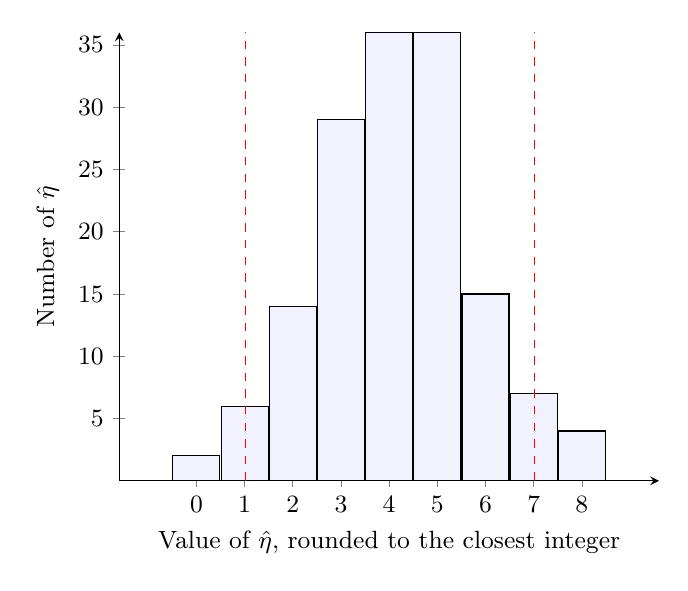
\begin{tikzpicture}[font=\small]
\begin{axis}[
ybar,
bar width=17pt,
xlabel={Value of $\hat{\eta}$, rounded to the closest integer},
ylabel={Number of $\hat{\eta}$},
ymin=0,
ytick={5,10,15,20,25,30,35,40},
xtick=data,
axis x line=bottom,
axis y line=left,
enlarge x limits=0.2,
]
\addplot[fill=myblue] coordinates {
    (0,2)
    (1, 6)
    (2, 14)
    (3, 29)
    (4, 36)
    (5, 36)
    (6, 15)
    (7, 7)
    (8, 4)
};
\end{axis}
\draw[dashed,red](1.6,0) -- (1.6,5.7);
\draw[dashed,red](5.27,0) -- (5.27,5.7);
\end{tikzpicture}
    \caption{Maximum likelihood estimate of 150 bootstrap samples, rounded to the closest integer. The red dashed lines represent the 5 and 95 percentiles.}
    \label{percentile_ci_example}
\end{figure}

The percentile method is simple to both understand and implement. However, these confidence intervals might be biased. Then, one could instead use approaches such as \textit{bias corrected and accelerated} intervals or \textit{approximate bootstrap confidence} intervals. For simplicity, we are in this report using the percentile confidence intervals. 

\newpage
\section{Problem Setup}

Small part about the inference and how we will do that.

%Then, something about that we first need the ideal observer solution. 
To be able to do that (describe that), we firstly need to find a model(?) for the Ideal Observer solution. In the specialization thesis we found one IO solution where we assumed that the number of red boxes is uniformly distributed with possible values $(0,1,2,3,4,5,7,8,9,10,11,12)$, where $6$ is not included here as one of the colours have to be in majority. 


Have one IO solution form the specialization thesis, generalising that one here to be able to have different prior for $\theta$. 

From the specialisation thesis we have the loss functions. Talk about the three different choices, and state the loss functions as you found them earlier. Then, say that you need those two probabilities, and say how you find them in this case 
\input{Sections/6-probabilities}
%\input{Sections/7-Trees}


\newpage
\bibliography{references.bib}


\end{document}
